
\documentclass[a4paper]{article}
\usepackage[utf8]{inputenc}
\usepackage{graphicx}
\usepackage{blindtext}
\usepackage{hyperref}
\usepackage{float}
\usepackage{caption}
\usepackage{subcaption}
\usepackage{indentfirst}
\usepackage{setspace}
\usepackage[font=footnotesize,labelfont=bf]{caption}

\setlength{\parindent}{6ex}
\setlength{\parskip}{0.2ex}
\renewcommand{\baselinestretch}{1.2}

\author{Emre Geçit, Baran Yancı}
\begin{document}

    \title{
\includegraphics[scale=0.2]{assets/ceng_400x400.png}\\ Software Requirements Specification for \\  \textbf{Afet Bilgi}}
    \maketitle

    \newpage
    \makeatletter
	\renewcommand\tableofcontents{%
		\null\hfill\textbf{\Large\contentsname}\hfill\null\par
		\@mkboth{\MakeUppercase\contentsname}{\MakeUppercase\contentsname}%
		\@starttoc{toc}%
	}
	\makeatother

    \tableofcontents
    \doublespacing

    \newpage

    \section{Introduction}

        Lorem ipsum dolor sit amet, consectetur adipiscing elit. Nullam eget libero sollicitudin justo vehicula venenatis quis ut eros. Proin vitae.

        \subsection{Purpose of the System}

        Lorem ipsum dolor sit amet, consectetur adipiscing elit. Nullam eget libero sollicitudin justo vehicula venenatis quis ut eros. Proin vitae.

            \subsection{Scope}

            Lorem ipsum dolor sit amet, consectetur adipiscing elit. Nullam eget libero sollicitudin justo vehicula venenatis quis ut eros. Proin vitae.

            \subsection{System Overview}

            Lorem ipsum dolor sit amet, consectetur adipiscing elit. Nullam eget libero sollicitudin justo vehicula venenatis quis ut eros. Proin vitae.

                \subsubsection{System Perspective}

                \begin{center}
                    \par
                    \begin{tabular}{cc}
                        \fbox{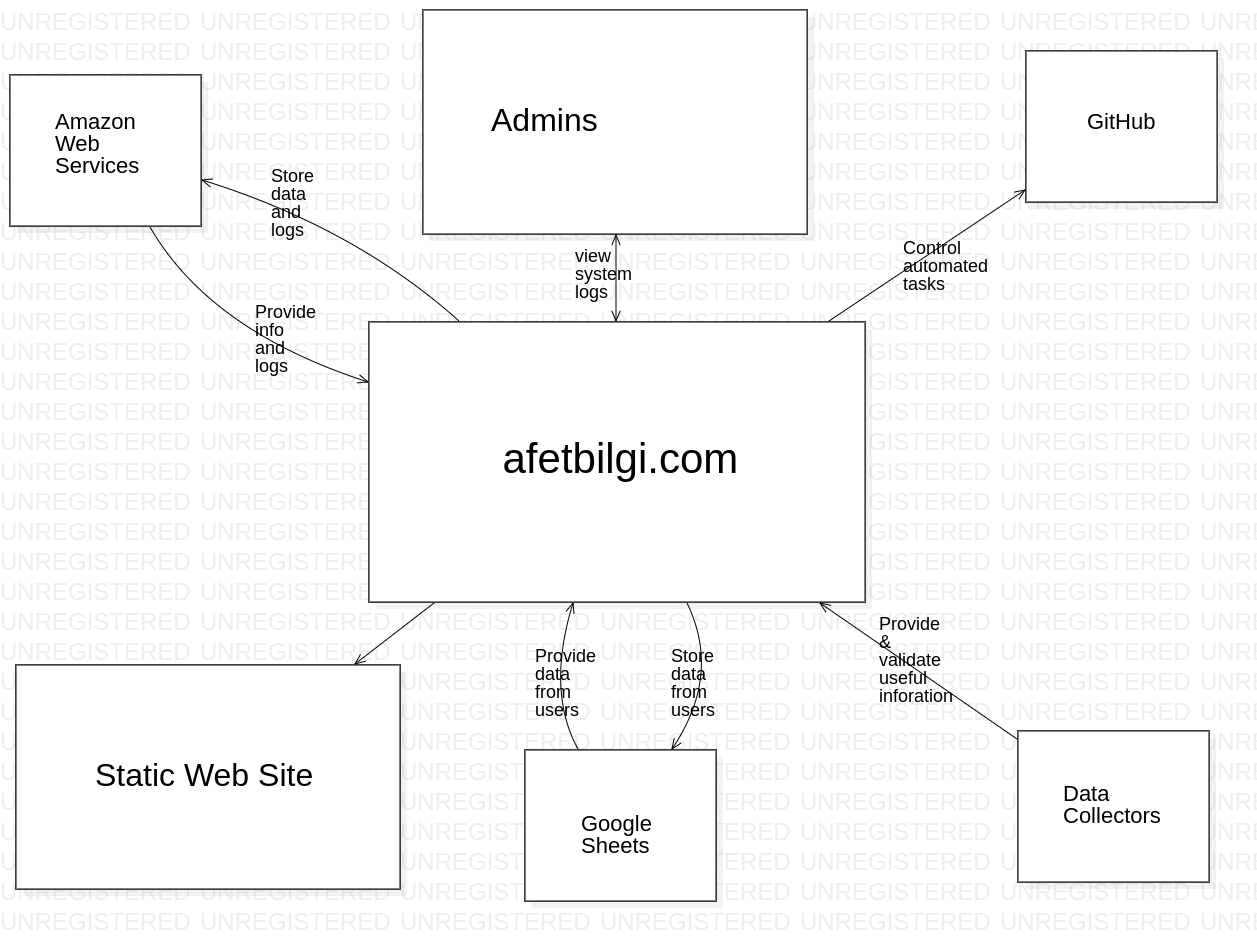
\includegraphics[width=1\linewidth]{./assets/context_diagram.png}}
                    \end{tabular}
                    \par
                    \captionof{figure}{Context Diagram}
                \end{center}

                The \verb*|afetbilgi.com| product is not an element of a larger system. The project is split into two main parts.
                The first part is the front-end of the website. The second part is the cloud services that is used to store and
                process the data. The front-end is a web application that is developed using TypeScript and the ReactJS framework.
                The front-end uses packages like MUI and is hosted on the static website \verb*|afetbilgi.com|. 
                For the cloud services, the project uses Amazon Web Services (AWS) and the serverless framework. Alongside AWS,
                GitHub Actions is used for continuous integration and continuous deployment (CI/CD). The cloud services process 
                the data and store it in a database. The data comes from individuals who enter and/or validate the data. The data
                is collected in Google Sheets and then processed by the cloud services. The cloud services are hosted on AWS.
                GitHub actions are also responsible for generating PDF files including information about affected areas, from the
                data in the database. The PDF files are then stored in the cloud services and can be accessed by the front-end.

                \subsubsection{System Functions}

                Lorem ipsum dolor sit amet, consectetur adipiscing elit. Nullam eget libero sollicitudin justo vehicula venenatis quis ut eros. Proin vitae.

                \subsubsection{Stakeholder Characteristics}

                Lorem ipsum dolor sit amet, consectetur adipiscing elit. Nullam eget libero sollicitudin justo vehicula venenatis quis ut eros. Proin vitae.

                \subsubsection{Limitations}

                Lorem ipsum dolor sit amet, consectetur adipiscing elit. Nullam eget libero sollicitudin justo vehicula venenatis quis ut eros. Proin vitae.

            \subsection{Definitions}

            Lorem ipsum dolor sit amet, consectetur adipiscing elit. Nullam eget libero sollicitudin justo vehicula venenatis quis ut eros. Proin vitae.

    \section{References}

    Lorem ipsum dolor sit amet, consectetur adipiscing elit. Nullam eget libero sollicitudin justo vehicula venenatis quis ut eros. Proin vitae.

    \section{Specific Requirements}

    Lorem ipsum dolor sit amet, consectetur adipiscing elit. Nullam eget libero sollicitudin justo vehicula venenatis quis ut eros. Proin vitae.

        \subsection{External Interfaces}

        Lorem ipsum dolor sit amet, consectetur adipiscing elit. Nullam eget libero sollicitudin justo vehicula venenatis quis ut eros. Proin vitae.

        \subsection{Functions}

        Lorem ipsum dolor sit amet, consectetur adipiscing elit. Nullam eget libero sollicitudin justo vehicula venenatis quis ut eros. Proin vitae.

        \subsection{Usability Requirements}

        Lorem ipsum dolor sit amet, consectetur adipiscing elit. Nullam eget libero sollicitudin justo vehicula venenatis quis ut eros. Proin vitae.

        \subsection{Performance Requirements}

        Lorem ipsum dolor sit amet, consectetur adipiscing elit. Nullam eget libero sollicitudin justo vehicula venenatis quis ut eros. Proin vitae.

        \subsection{Logical Database Requirements}

        Lorem ipsum dolor sit amet, consectetur adipiscing elit. Nullam eget libero sollicitudin justo vehicula venenatis quis ut eros. Proin vitae.

        \subsection{Design Constraints}

        Lorem ipsum dolor sit amet, consectetur adipiscing elit. Nullam eget libero sollicitudin justo vehicula venenatis quis ut eros. Proin vitae.

        \subsection{System Attributes}

        Lorem ipsum dolor sit amet, consectetur adipiscing elit. Nullam eget libero sollicitudin justo vehicula venenatis quis ut eros. Proin vitae.

        \subsection{Supporting Information}

        Lorem ipsum dolor sit amet, consectetur adipiscing elit. Nullam eget libero sollicitudin justo vehicula venenatis quis ut eros. Proin vitae.

    \section{Suggestions for Future Work}

    Lorem ipsum dolor sit amet, consectetur adipiscing elit. Nullam eget libero sollicitudin justo vehicula venenatis quis ut eros. Proin vitae.

        \subsection{System Perspective}

        Lorem ipsum dolor sit amet, consectetur adipiscing elit. Nullam eget libero sollicitudin justo vehicula venenatis quis ut eros. Proin vitae.

        \subsection{External Interfaces}

        Lorem ipsum dolor sit amet, consectetur adipiscing elit. Nullam eget libero sollicitudin justo vehicula venenatis quis ut eros. Proin vitae.

        \subsection{Functions}

        Lorem ipsum dolor sit amet, consectetur adipiscing elit. Nullam eget libero sollicitudin justo vehicula venenatis quis ut eros. Proin vitae.

        \subsection{Usability Requirements}

        Lorem ipsum dolor sit amet, consectetur adipiscing elit. Nullam eget libero sollicitudin justo vehicula venenatis quis ut eros. Proin vitae.

        \subsection{Performance Requirements}

        Lorem ipsum dolor sit amet, consectetur adipiscing elit. Nullam eget libero sollicitudin justo vehicula venenatis quis ut eros. Proin vitae.

        \subsection{Logical Database Requirements}

        Lorem ipsum dolor sit amet, consectetur adipiscing elit. Nullam eget libero sollicitudin justo vehicula venenatis quis ut eros. Proin vitae.

        \subsection{Design Constraints}

        Lorem ipsum dolor sit amet, consectetur adipiscing elit. Nullam eget libero sollicitudin justo vehicula venenatis quis ut eros. Proin vitae.

        \subsection{System Attributes}

        Lorem ipsum dolor sit amet, consectetur adipiscing elit. Nullam eget libero sollicitudin justo vehicula venenatis quis ut eros. Proin vitae.

        \subsection{Supporting Information}

        Lorem ipsum dolor sit amet, consectetur adipiscing elit. Nullam eget libero sollicitudin justo vehicula venenatis quis ut eros. Proin vitae.



\end{document}